\documentclass[12pt, titlepage]{article}

\usepackage{fullpage}
\usepackage[round]{natbib}
\usepackage{multirow}
\usepackage{booktabs}
\usepackage{tabularx}
\usepackage{graphicx}
\usepackage{float}
\usepackage{hyperref}
\hypersetup{
    colorlinks,
    citecolor=black,
    filecolor=black,
    linkcolor=red,
    urlcolor=blue
}
\usepackage[round]{natbib}

\newcounter{acnum}
\newcommand{\actheacnum}{AC\theacnum}
\newcommand{\acref}[1]{AC\ref{#1}}

\newcounter{ucnum}
\newcommand{\uctheucnum}{UC\theucnum}
\newcommand{\uref}[1]{UC\ref{#1}}

\newcounter{mnum}
\newcommand{\mthemnum}{M\themnum}
\newcommand{\mref}[1]{M\ref{#1}}

\usepackage{titlesec}

\setcounter{secnumdepth}{4}

\title{SE 3XA3: Software Requirements Specification}

\author{Team 10, MacLunky
		\\ Albert Zhou, zhouj103
		\\Abeer Al-Yasiri, alyasira
		\\ Niyatha Rangarajan, rangaran
}


\date{April 12, 2021}

%\input{../../Comments}

\begin{document}

\maketitle

\pagenumbering{roman}
\tableofcontents
\listoftables
\listoffigures

\begin{table}[hp]
\caption{Revision History} \label{TblRevisionHistory}
\begin{tabularx}{\textwidth}{llX}
\toprule
\textbf{Date} & \textbf{Developer(s)} & \textbf{Change}\\
\midrule
March 11, 2021 & Albert, Abeer, Niyatha & Version 0 made\\
% \midrule
% April 1, 2021 & Albert & Entity secrets, collectable modules\\
\midrule
April 12, 2021 & Albert, Abeer, Niyatha & Revision 1 modifications\\
\bottomrule
\end{tabularx}
\end{table}


\newpage

\pagenumbering{arabic}

\section{Introduction}

Decomposing a system into modules is a commonly accepted approach to developing
software.  A module is a work assignment for a programmer or programming
team~\citep{ParnasEtAl1984}.  We advocate a decomposition
based on the principle of information hiding~\citep{Parnas1972a}.  This
principle supports design for change, because the ``secrets'' that each module
hides represent likely future changes.  Design for change is valuable in SC,
where modifications are frequent, especially during initial development as the
solution space is explored.  

Our design follows the rules layed out by \citet{ParnasEtAl1984}, as follows:
\begin{itemize}
\item System details that are likely to change independently should be the
  secrets of separate modules.
\item Each data structure is used in only one module.
\item Any other program that requires information stored in a module's data
  structures must obtain it by calling access programs belonging to that module.
\end{itemize}

After completing the first stage of the design, the Software Requirements
Specification (SRS), the Module Guide (MG) is developed~\citep{ParnasEtAl1984}. The MG
specifies the modular structure of the system and is intended to allow both
designers and maintainers to easily identify the parts of the software.  The
potential readers of this document are as follows:

\begin{itemize}
\item New project members: This document can be a guide for a new project member
  to easily understand the overall structure and quickly find the
  relevant modules they are searching for.
\item Maintainers: The hierarchical structure of the module guide improves the
  maintainers' understanding when they need to make changes to the system. It is
  important for a maintainer to update the relevant sections of the document
  after changes have been made.
\item Designers: Once the module guide has been written, it can be used to
  check for consistency, feasibility and flexibility. Designers can verify the
  system in various ways, such as consistency among modules, feasibility of the
  decomposition, and flexibility of the design.
\end{itemize}

The rest of the document is organized as follows. Section
\ref{SecChange} lists the anticipated and unlikely changes of the software
requirements. Section \ref{SecMH} summarizes the module decomposition that
was constructed according to the likely changes. Section \ref{SecConnection}
specifies the connections between the software requirements and the
modules. Section \ref{SecMD} gives a detailed description of the
modules. Section \ref{SecTM} includes two traceability matrices. One checks
the completeness of the design against the requirements provided in the SRS. The
other shows the relation between anticipated changes and the modules. Section
\ref{SecUse} describes the use relation between modules.

\section{Anticipated and Unlikely Changes} \label{SecChange}

This section lists possible changes to the system. According to the likeliness
of the change, the possible changes are classified into two
categories. Anticipated changes are listed in Section \ref{SecAchange}, and
unlikely changes are listed in Section \ref{SecUchange}.

\subsection{Anticipated Changes} \label{SecAchange}

Anticipated changes are the source of the information that is to be hidden
inside the modules. Ideally, changing one of the anticipated changes will only
require changing the one module that hides the associated decision. The approach
adapted here is called design for change.

\begin{description}
\item[\refstepcounter{acnum} \actheacnum \label{acHardware}:] The specific
  hardware and OS on which the software is running.
\item[\refstepcounter{acnum} \actheacnum \label{acInput}:] The format of the input data the player uses for controls.
\item [\refstepcounter{acnum} \actheacnum \label{acWindow}:] The user controls the size of the game window. 
\item [\refstepcounter{acnum} \actheacnum \label{acScreen}:] Adapting new game levels by changing the game screen as the player progress in the game.
\item [\refstepcounter{acnum} \actheacnum \label{acObject}:] The size and image of game objects.
\item [\refstepcounter{acnum} \actheacnum \label{acSpeed}:] The player's speed. 
\item [\refstepcounter{acnum} \actheacnum \label{acSpeed2}:] The speed of the interactive moving objects in the game.
\item [\refstepcounter{acnum} \actheacnum \label{acScore}:] The player scoring system and health points. 
\item [\refstepcounter{acnum} \actheacnum \label{acAction}:] The player movement and attack mechanisms. 
\item [\refstepcounter{acnum} \actheacnum \label{acWin}:] The winning criteria of the game. 
\item [\refstepcounter{acnum} \actheacnum \label{acPlayer}:] The player character features such as shape, size, and theme. 
\end{description}

\subsection{Unlikely Changes} \label{SecUchange}

The module design should be as general as possible. However, a general system is
more complex. Sometimes this complexity is not necessary. Fixing some design
decisions at the system architecture stage can simplify the software design. If
these decision should later need to be changed, then many parts of the design
will potentially need to be modified. Hence, it is not intended that these
decisions will be changed.

\begin{description}
\item[\refstepcounter{ucnum} \uctheucnum \label{ucIO}:] Input/Output devices
  (Input: File and/or Keyboard, Output: File, Memory, and/or Screen).
\item[\refstepcounter{ucnum} \uctheucnum \label{ucInput}:] There will always be
  a source of input data external to the software.
\item[\refstepcounter{ucnum} \uctheucnum \label{ucObject}:] The behaviour of the game's interactive objects. 
\item[\refstepcounter{ucnum} \uctheucnum \label{ucOptions}:] The control options used by the player. 
\item[\refstepcounter{ucnum} \uctheucnum \label{ucScreen}:] The types of screen display of the game.
\item[\refstepcounter{ucnum} \uctheucnum \label{ucScore}:] The input to the scoring system saving procedure. 
\item[\refstepcounter{ucnum} \uctheucnum \label{ucPlayer}:] The number of players in one game run. 
\item[\refstepcounter{ucnum} \uctheucnum \label{ucSound}:] Adding player movement and game environment sounds.
\end{description}

\section{Module Hierarchy} \label{SecMH}

This section provides an overview of the module design. Modules are summarized
in a hierarchy decomposed by secrets in Table \ref{TblMH}. The modules listed
below, which are leaves in the hierarchy tree, are the modules that will
actually be implemented.

\begin{description}
\item [\refstepcounter{mnum} \mthemnum \label{mHH1}:] Display Module
\item [\refstepcounter{mnum} \mthemnum \label{mHH2}:] Input Controls Module
\item [\refstepcounter{mnum} \mthemnum \label{mBH1}:] Player Module
\item [\refstepcounter{mnum} \mthemnum \label{mBH2}:] Entities Module
    {\color{red}\begin{enumerate}
        \item \label{mBH2.1} Entity Module
        \item \label{mBH2.2} Collectable Module
        \item \label{mBH2.3} Treasure Module
        \item \label{mBH2.4} Gold Module
        \item \label{mBH2.5} Sapphire Module
        \item \label{mBH2.6} Emerald Module
        \item \label{mBH2.7} Ruby Module
        \item \label{mBH2.8} Diamond Module
        \item \label{mBH2.9} BombPile Module
        \item \label{mBH2.10} RopePile Module
        \item \label{mBH2.11} Sign Module
        \item \label{mBH2.12} Explosion Module
        \item \label{mBH2.13} Rope Module
        \item \label{mBH2.14} Throwable Module
        \item \label{mBH2.15} Chest Module
        \item \label{mBH2.16} Bomb Module
        \item \label{mBH2.17} EmptyHand Module
        \item \label{mBH2.18} Enemy Module
        \item \label{mBH2.19} Snake Module
        \item \label{mBH2.20} Spider Module
        \item \label{mBH2.21} Trap Module
        \item \label{mBH2.22} ArrowTrap Module
        \item \label{mBH2.23} Arrow Module
        \item \label{mBH2.24} Spikes Module
        \item \label{mBH2.25} Weapon Module
        \item \label{mBH2.26} Whip Module
        %\item \label{mBH2.19} Module
    \end{enumerate}}
\item [\refstepcounter{mnum} \mthemnum \label{mBH3}:] Game State Module
\item [\refstepcounter{mnum} \mthemnum \label{mBH4}:] Game Level Module
\item [\refstepcounter{mnum} \mthemnum \label{mSD1}:] Overlap Module
\item [\refstepcounter{mnum} \mthemnum \label{mSD2}:] Gravity Module
\end{description}


\begin{table}[H]
\centering
\begin{tabular}{p{0.3\textwidth} p{0.6\textwidth}}
\toprule
\textbf{Level 1} & \textbf{Level 2}\\
\midrule

{Hardware-Hiding Module} & Display \\
& Input Controls \\
\midrule

\multirow{4}{0.3\textwidth}{Behaviour-Hiding Module} & Player \\
& Entities \\
& \textcolor{red}{Entity} \\
& \textcolor{red}{Collectable} \\
& \textcolor{red}{Treasure} \\
& \textcolor{red}{Gold} \\
& \textcolor{red}{Sapphire} \\
& \textcolor{red}{Emerald} \\
& \textcolor{red}{Ruby} \\
& \textcolor{red}{Diamond} \\
& \textcolor{red}{BombPile} \\
& \textcolor{red}{RopePile} \\
& \textcolor{red}{Gold} \\
& \textcolor{red}{Gem} \\
& \textcolor{red}{Sign}\\
& \textcolor{red}{Explosion}\\
& \textcolor{red}{Rope}\\
& \textcolor{red}{Throwable}\\
& \textcolor{red}{Chest}\\
& \textcolor{red}{Bomb}\\
& \textcolor{red}{EmptyHand}\\
& \textcolor{red}{Enemy}\\
& \textcolor{red}{Snake}\\
& \textcolor{red}{Spider}\\
& \textcolor{red}{Trap}\\
& \textcolor{red}{ArrowTrap}\\
& \textcolor{red}{Arrow}\\
& \textcolor{red}{Spikes}\\
& \textcolor{red}{Weapon}\\
& \textcolor{red}{Whip}\\
& Game State \\
& Game Level\\
\midrule


\multirow{2}{0.3\textwidth}{Software Decision Module}
& Overlap\\
& Gravity\\
\bottomrule

\end{tabular}
\caption{Module Hierarchy}
\label{TblMH}
\end{table}

\section{Connection Between Requirements and Design} \label{SecConnection}

The design of the system is intended to satisfy the requirements developed in
the SRS. In this stage, the system is decomposed into modules. The connection
between requirements and modules is listed in Table \ref{TblRT}.

\section{Module Decomposition} \label{SecMD}

Modules are decomposed according to the principle of ``information hiding''
proposed by \citet{ParnasEtAl1984}. The \emph{Secrets} field in a module
decomposition is a brief statement of the design decision hidden by the
module. The \emph{Services} field specifies \emph{what} the module will do
without documenting \emph{how} to do it. For each module, a suggestion for the
implementing software is given under the \emph{Implemented By} title. If the
entry is \emph{OS}, this means that the module is provided by the operating
system or by standard programming language libraries.  Also indicate if the
module will be implemented specifically for the software.

Only the leaf modules in the hierarchy have to be implemented. If a dash (\emph{--}) is shown, this means that the module is not a leaf and will not have to be implemented. Whether or not this module is implemented depends on the programming language
selected.

\subsection{Hardware Hiding Modules}

% \begin{description}
% \item[Secrets:]The data structure and algorithm used to implement the virtual
%   hardware.
% \item[Services:]Serves as a virtual hardware used by the rest of the
%   system. This module provides the interface between the hardware and the
%   software. So, the system can use it to display outputs or to accept inputs.
% \item[Implemented By:] OS
% \end{description}

\subsubsection{Display Module \mref{mHH1}}

\begin{description}
\item[Secrets:] Loads the ui of the game involving the display of the map, entities placed on the map and the player that the user controls. 
\item[Services:] The input takes all game entities and player images to be displayed. Output shows a visual rendition of the game after various in-game interactions. Adjusts on screen images to represent a game object in motion.
\item[Implemented By:] Original project
\end{description}

\subsubsection{Input Controls Module \mref{mHH2}}

\begin{description}
\item[Secrets:] The mechanism to connect user keyboard inputs with object creation/interaction and  movement on the game map screen.
\item[Services:] The output translates (for a given frame rate) the game object's movement that is their game map coordinates based on the key provided. The output could also generate map entities that subsequently interact with the player. Finally the key inputs can also allow the player to have access to defense mechanism while interacting with other map objects.
\item[Implemented By:] Original project
\end{description}

\subsection{Behaviour-Hiding Module}

% \begin{description}
% \item[Secrets:]The contents of the required behaviours.
% \item[Services:]Includes programs that provide externally visible behaviour of
%   the system as specified in the software requirements specification (SRS)
%   documents. This module serves as a communication layer between the
%   hardware-hiding module and the software decision module. The programs in this
%   module will need to change if there are changes in the SRS.
% \item[Implemented By:] --
% \end{description}

\subsubsection{Player Module \mref{mBH1}}

\begin{description}
\item[Secrets:] The module containing the state and characteristics of the player character.
\item[Services:] Provides movement, interactions with entities, resource tracking, and resource use for the player character.
\item[Implemented By:] Original Project
\end{description}

\subsubsection{Entities Module \mref{mBH2}}

\begin{description}
\item[Secrets:] The module containing the state data of all entities found in the game.
% \item[Services:] Provides all types of entities found in the game and their interactions with the player, themselves, and their environment.
\item[Services:] Provides the data of all types of entities found in the game.
\item[Implemented By:] Original project
\end{description}

{\color{red}
\paragraph{Entity Module M4.\ref{mBH2.1}}
\begin{description}
\item[Secrets:] Entity functions.
\item[Services:] Provides functions for entity entities. 
\item[Implemented By:] Albert Zhou
\end{description}

\paragraph{Collectable Module M4.\ref{mBH2.2}}
\begin{description}
\item[Secrets:] Entity functions.
\item[Services:] Provides functions for collectable entities. 
\item[Implemented By:] Albert Zhou
\end{description}

\paragraph{Treasure Module M4.\ref{mBH2.3}}
\begin{description}
\item[Secrets:] Entity functions.
\item[Services:] Provides functions for treasure entities. 
\item[Implemented By:] Albert Zhou
\end{description}

\paragraph{Gold Module M4.\ref{mBH2.4}}
\begin{description}
\item[Secrets:] Gold functions.
\item[Services:] Provides functions for gold entities. 
\item[Implemented By:] Albert Zhou
\end{description}

\paragraph{Sapphire Module M4.\ref{mBH2.5}}
\begin{description}
\item[Secrets:] Sapphire functions.
\item[Services:] Provides functions for sapphire entities. 
\item[Implemented By:] Albert Zhou
\end{description}

\paragraph{Emerald Module M4.\ref{mBH2.6}}
\begin{description}
\item[Secrets:] Emerald functions.
\item[Services:] Provides functions for emerald entities. 
\item[Implemented By:] Albert Zhou
\end{description}

\paragraph{Ruby Module M4.\ref{mBH2.7}}
\begin{description}
\item[Secrets:] Ruby functions.
\item[Services:] Provides functions for ruby entities. 
\item[Implemented By:] Albert Zhou
\end{description}

\paragraph{Diamond Module M4.\ref{mBH2.8}}
\begin{description}
\item[Secrets:] Diamond functions.
\item[Services:] Provides functions for diamond entities. 
\item[Implemented By:] Albert Zhou
\end{description}

\paragraph{BombPile Module M4.\ref{mBH2.9}}
\begin{description}
\item[Secrets:] BombPile functions.
\item[Services:] Provides functions for bombPile entities. 
\item[Implemented By:] Albert Zhou
\end{description}

\paragraph{RopPile Module M4.\ref{mBH2.10}}
\begin{description}
\item[Secrets:] RopPile functions.
\item[Services:] Provides functions for RopPile entities. 
\item[Implemented By:] Albert Zhou
\end{description}

\paragraph{Sign Module M4.\ref{mBH2.11}}
\begin{description}
\item[Secrets:] Sign functions.
\item[Services:] Provides functions for sign entities. 
\item[Implemented By:] Original project
\end{description}

\paragraph{Explosion Module M4.\ref{mBH2.12}}
\begin{description}
\item[Secrets:] Explosion functions.
\item[Services:] Provides functions for explosion entities. 
\item[Implemented By:] Albert Zhou
\end{description}

\paragraph{Rope Module M4.\ref{mBH2.13}}
\begin{description}
\item[Secrets:] Rope functions.
\item[Services:] Provides functions for rope entities. 
\item[Implemented By:] Albert Zhou
\end{description}

\paragraph{Throwable Module M4.\ref{mBH2.14}}
\begin{description}
\item[Secrets:] Throwable functions.
\item[Services:] Provides functions for throwing and moving entities. 
\item[Implemented By:] Albert Zhou
\end{description}

\paragraph{Chest Module M4.\ref{mBH2.15}}
\begin{description}
\item[Secrets:] Chest functions.
\item[Services:] Provides functions for chest entities. 
\item[Implemented By:] Albert Zhou
\end{description}

\paragraph{Bomb Module M4.\ref{mBH2.16}}
\begin{description}
\item[Secrets:] Bomb functions.
\item[Services:] Provides functions for bomb entities. 
\item[Implemented By:] Albert Zhou
\end{description}

\paragraph{EmptyHand Module M4.\ref{mBH2.17}}
\begin{description}
\item[Secrets:] EmptyHand functions.
\item[Services:] Provides functions for emptyHand entities. 
\item[Implemented By:] Albert Zhou
\end{description}

\paragraph{Enemy Module M4.\ref{mBH2.18}}
\begin{description}
\item[Secrets:] Enemy functions.
\item[Services:] Provides functions for enemy entities. 
\item[Implemented By:] Niyatha Rangarajan
\end{description}

\paragraph{Snake Module M4.\ref{mBH2.19}}
\begin{description}
\item[Secrets:] Snake functions.
\item[Services:] Provides functions for snake entities. 
\item[Implemented By:] Niyatha Rangarajan
\end{description}

\paragraph{Spider Module M4.\ref{mBH2.20}}
\begin{description}
\item[Secrets:] Spider functions.
\item[Services:] Provides functions for spider entities. 
\item[Implemented By:] Niyatha Rangarajan
\end{description}

\paragraph{Trap Module M4.\ref{mBH2.21}}
\begin{description}
\item[Secrets:] Trap functions.
\item[Services:] Provides functions for trap entities. 
\item[Implemented By:] Abeer Al-Yasiri
\end{description}

\paragraph{ArrowTrap Module M4.\ref{mBH2.22}}
\begin{description}
\item[Secrets:] ArrowTrap functions.
\item[Services:] Provides functions for arrowTrap entities. 
\item[Implemented By:] Abeer Al-Yasiri
\end{description}

\paragraph{Arrow Module M4.\ref{mBH2.23}}
\begin{description}
\item[Secrets:] Arrow functions.
\item[Services:] Provides functions for arrow entities. 
\item[Implemented By:] Abeer Al-Yasiri
\end{description}

\paragraph{Spikes Module M4.\ref{mBH2.24}}
\begin{description}
\item[Secrets:] Spikes functions.
\item[Services:] Provides functions for spikes entities. 
\item[Implemented By:] Abeer Al-Yasiri
\end{description}

\paragraph{Weapon Module M4.\ref{mBH2.25}}
\begin{description}
\item[Secrets:] Weapon functions.
\item[Services:] Provides functions for weapon entities. 
\item[Implemented By:] Albert Zhou
\end{description}

\paragraph{Whip Module M4.\ref{mBH2.26}}
\begin{description}
\item[Secrets:] Whip functions.
\item[Services:] Provides functions for whip entities. 
\item[Implemented By:] Albert Zhou
\end{description}
}

\subsubsection{Game State Module \mref{mBH3}}

\begin{description}
\item[Secrets:] The module for provoking changes in the game with respect to time..
\item[Services:] Provides game initialization and timing for the player and entities.
\item[Implemented By:] Original project
\end{description}

\subsubsection{Game Level Module \mref{mBH4}}

\begin{description}
\item[Secrets:] The module responsible for creating and storing game levels.
\item[Services:] Provides level generation from map files containing the types and locations of all blocks and entities.
\item[Implemented By:] Original project
\end{description}


\subsection{Software Decision Module}

% \begin{description}
% \item[Secrets:] The design decision based on mathematical theorems, physical
%   facts, or programming considerations. The secrets of this module are
%   \emph{not} described in the SRS.
% \item[Services:] Includes data structure and algorithms used in the system that
%   do not provide direct interaction with the user. 
%   % Changes in these modules are more likely to be motivated by a desire to
%   % improve performance than by externally imposed changes.
% \item[Implemented By:] --
% \end{description}

\subsubsection{Overlap Module \mref{mSD1}}
\begin{description}
\item[Secrets:] The mechanism for detecting the collision between two interactive objects in the game. 
\item[Services:] Detects if two objects are colliding at the same position and time of action. The module takes static inputs of objects state in the game and returns a Boolean of the collision state of the two input objects. The output of the module is used to make game state change decisions to the interacted objects. 
\item[Implemented By:] Albert Zhou
\end{description}

\subsubsection{Gravity Module \mref{mSD2}}
\begin{description}
\item[Secrets:] The control mechanism of representing the affect of gravity in the game.
\item[Services:] Affects how interactive objects in the game descends in open space. It determines the speed at which objects fall from various heights in the game. The effects of the modules on the game's objects are used in other modules to make state change decisions for the effected objects.
\item[Implemented By:] Original project
\end{description}

\section{Traceability Matrix} \label{SecTM}

This section shows two traceability matrices: between the modules and the
requirements and between the modules and the anticipated changes.

% the table should use mref, the requirements should be named, use something
% like fref
\begin{table}[H]
\centering
\begin{tabular}{p{0.2\textwidth} p{0.6\textwidth}}
\toprule
\textbf{Req.} & \textbf{Modules}\\
\midrule
R1-R2 & \mref{mBH3}\\
R3-R5 & \mref{mHH1}\\
R6-R15,R34 &  \mref{mHH2}, \mref{mBH1}, \mref{mSD2}, \mref{mSD1}\\
R16-R19 & M4.\mref{mBH2.12},  M4.\mref{mBH2.16}, \mref{mSD2}, \mref{mSD1}, M4.\ref{mBH2.16}\\
R20-R24 & \mref{mBH1}, M4.\mref{mBH2.13}, \mref{mSD1}\\
R25-R27 & \mref{mBH1}, M4.\mref{mBH2.25}, \mref{mSD1}\\
R28-R30 & \mref{mBH1}, \mref{mSD2}\\
R31-R33 & \mref{mBH2.3}\\
R35-R38,R49 & M4.\mref{mBH2.18}, \mref{mSD1}\\
R39-R48, 91 & M4.\mref{mBH2.2} - 7, M4.\mref{mBH2.15}\\
R50-54 & M4.\mref{mBH2.19}, \mref{mSD1}\\
R55-62 & M4.\mref{mBH2.20}, \mref{mSD1}\\
R39-R48 & \mref{mBH2}, \mref{mSD1}\\
R63 & M4.\mref{mBH2.21}\\
R64-R71, 90 & M4.\mref{mBH2.22}, M4.\mref{mBH2.23}, \mref{mSD1}\\
R72-R73 & M4.\mref{mBH2.24}\\
R74-R77 & \mref{mHH1}, \mref{mBH1}\\
R78-R84 & \mref{mBH4}\\
R85-R87 & M4.\mref{mBH2.11}\\
R88 & M4.\mref{mBH2.9}\\
R89 & M4.\mref{mBH2.10}\\

\bottomrule
\end{tabular}
\caption{Trace Between Requirements and Modules}
\label{TblRT}
\end{table}

\begin{table}[H]
\centering
\begin{tabular}{p{0.2\textwidth} p{0.6\textwidth}}
\toprule
\textbf{Req.} & \textbf{Modules}\\
\midrule
NFR1 & All modules\\
NFR2 & All modules\\
NFR3 & \mref{mBH3}\\
NFR4 & \mref{mBH1}\\
NFR5 & \mref{mBH3}\\
NFR6 & \mref{mBH1}\\
NFR7 & \mref{mBH1}\\
NFR8 & \mref{mBH3}\\
NFR9 & \mref{mBH3}\\
NFR10 & All modules\\
NFR11 & All modules\\
NFR12 & All modules\\
NFR13 & All modules\\
NFR14 & All modules\\
NFR15 & All modules\\
NFR16 & All modules\\
NFR17 & All modules\\
NFR18 & All modules\\
NFR19 & \mref{mBH4}\\
NFR20 & \mref{mBH1}\\
NFR21 & All modules\\
NFR22 & All modules\\
NFR23 & \mref{mBH1}\\
NFR24 & \mref{mBH1}\\
\bottomrule
\end{tabular}
\caption{Trace Between Non Functional Requirements and Modules}
\label{TblNFRT}
\end{table}

\begin{table}[H]
\centering
\begin{tabular}{p{0.2\textwidth} p{0.6\textwidth}}
\toprule
\textbf{AC} & \textbf{Modules}\\
\midrule
\acref{acHardware} & \mref{mHH1}\\
\acref{acInput} & \mref{mHH2}\\
\acref{acWindow} & \mref{mHH1}\\
\acref{acScreen} & \mref{mBH4}\\
\acref{acObject} & \mref{mBH2}\\
\acref{acSpeed} & \mref{mBH1}\\
\acref{acSpeed2} & \mref{mBH2}\\
\acref{acScore} & \mref{mBH3}\\
\acref{acAction} & \mref{mBH1}\\
\acref{acWin} & \mref{mBH3}\\
\acref{acPlayer} & \mref{mBH1}\\
%\acref{acPlot} & \mref{mPlot}\\
\bottomrule
\end{tabular}
\caption{Trace Between Anticipated Changes and Modules}
\label{TblACT}
\end{table}

\section{Use Hierarchy Between Modules} \label{SecUse}

In this section, the uses hierarchy between modules is
provided. \citet{Parnas1978} said of two programs A and B that A {\em uses} B if
correct execution of B may be necessary for A to complete the task described in
its specification. That is, A {\em uses} B if there exist situations in which
the correct functioning of A depends upon the availability of a correct
implementation of B.  Figure \ref{FigUH} illustrates the use relation between
the modules. It can be seen that the graph is a directed acyclic graph
(DAG). Each level of the hierarchy offers a testable and usable subset of the
system, and modules in the higher level of the hierarchy are essentially simpler
because they use modules from the lower levels.

\begin{figure}[H]
\centering
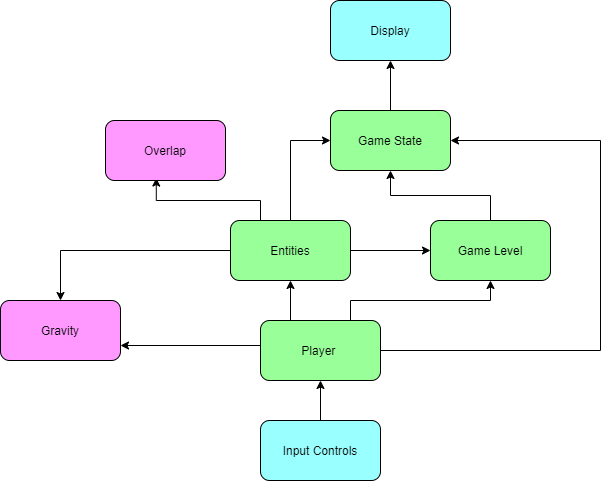
\includegraphics[width=0.7\textwidth]{UsesHierarchy.png}
\caption{Use hierarchy among modules}
\label{FigUH}
\end{figure}

\begin{figure}[H]
\centering
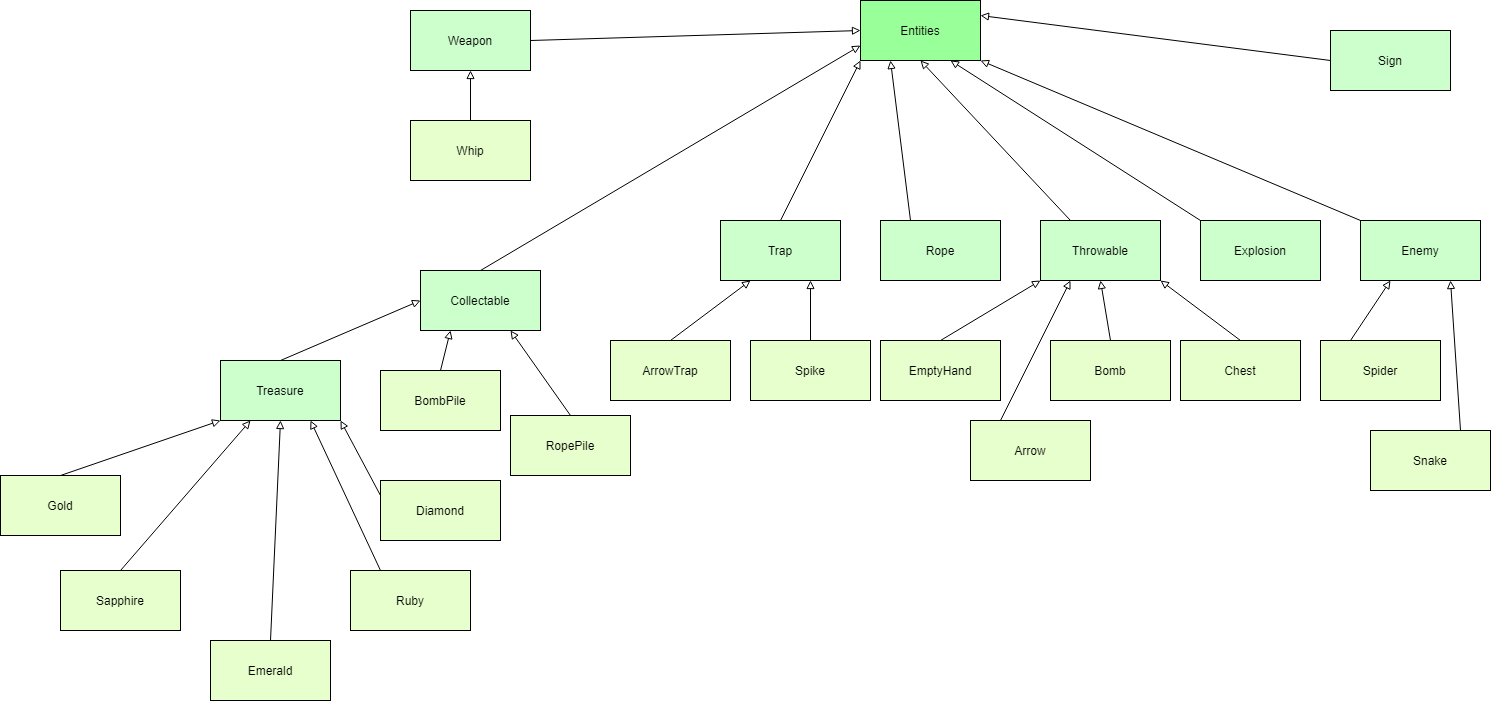
\includegraphics[width=0.7\textwidth]{entities.png}
\caption{Use hierarchy among entity modules}
\label{FigUHE}
\end{figure}

%\section*{References}

\bibliographystyle {plainnat}
\bibliography {ModuleGuide}

\end{document}
